% partie logiciel:
% 2D

% 3D 1: intersection de demi-espaces -> associer plane + inter pour AD (lien avec AD), type de nombre
% 3D 2: inclusion-exclusion
% -> environ 3 pages + bouts de codes

\chapter{Introduction}

Point clouds are useful objects in all the domains related to computer-based
processing like image processing or computer graphics because they can
represent any 3D object by only storing coordinates of points on this object. We
can obtain them from, for example, digitizing device such as a 3D scanner. A 3D
scanner is a tool which can scan a real 3D object, a surface, using for example
lasers. It samples points on the object to obtain a numeric version of the
scanned object. They can be then used to create more complex and complete models
like meshes which can be used in a software. For example, we can use surface
reconstruction algorithms like \cite{alexa2003computing}. But an important
problem arises from this technique: since the 3D scanner is a physics-based
tool, error will be made during the measurement: the resulting point cloud will
be noisy. We will be interested in removing this noise from the point cloud: we
call this technique denoising or smoothing.

There is also an other issue: we only deal with points and so we can not use all
the techniques developed in image processing like the Fourier transform,
wavelets... This is because, when we have an image, we can parametrize it
easily, for example, as a grid of pixels.  When we have a mesh, we have a kind
of parametrization but when we have only points, we do not have such
parametrization.

Several ways already exist to remove this noise and so to smooth point clouds.
Some are based on Computer Vision algorithms and some are more Computational
Geometry-based.

\begin{itemize}
    \item \textit{Gaussian / Laplacian smoothing}: replace a vertex by an other point
        computed along the nearest neighbours of the vertex. For the Laplacian
        case, the new point is the average of the neighbours (see
        \cite{vollmer1999improved}).
    \item \textit{Jet fitting} (see \cite{cazals2005estimating}): a jet is a truncated
        Taylor expansion. Such jets are fitted around points. Jet smoothing
        operates by projecting the input points on an estimated smooth
        parametric surface (the so-called jet surface). Jets are good because
        they intrinsically contain differential information such as normal,
        curvature...
    \item \textit{Bilateral smoothing} (see \cite{huang2013edge}): it is a way to do a
        smoothing while taking account the sharp edges present in the point set.
\end{itemize}

During this internship, we will use the following idea: move each point in the
direction of the inward normal by a quantity related to the mean curvature at
that point. The more curved is the surface, the more important the displacement
will be. The evolution of the surface can be modelled using a partial
differential equation. We will obtain a family of surfaces indexed by the time,
this family is called the mean curvature flow (MCF) of the initial surface.

The MCF can be seen as the geometric equivalent of the heat equation: indeed,
the Laplacian is replaced by the mean curvature vector. Both of them are sums of
eigenvalues of some matrices: the Hessian for the first one and the Shape
operator for the second.

% TODO: heat

The MCF is well-known for its smoothing properties (see
\cite{ciomaga2010level}). For example, the figure
\ref{fig:mean-curvature-flow-ex} is an illustration of the mean curvature flow
on a noised surface (extracted from \cite{clarenz2000anisotropic}).

\begin{figure}[h]
    \centering
    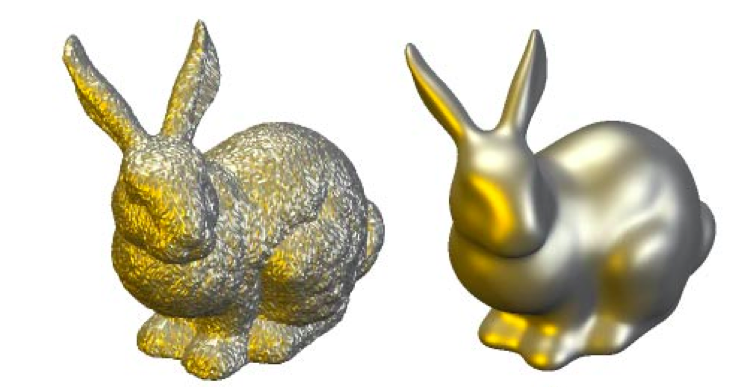
\includegraphics[scale=0.3]{img/mean-curvature-flow-rabbit}
    \caption{Mean curvature flow on a noised surface}
    \label{fig:mean-curvature-flow-ex}
\end{figure}

We will show in the last chapter of this report that this flow is linked to the
variation of the area of the surface. If we try to transform the surface while
minimizing the area, we will obtain the same evolution as the one given by the
MCF. But let us recall that we only know points sampled on a surface and not the
underlying surface. So, we will need a way to compute the area without knowing
the original surface. A common way of doing it is to consider the volume of the
union of balls centered on the points of the cloud.  We will show that this
quantity is proportional, under some sampling conditions, to the area of the
underlying surface.

Now that we have our energy, we need to minimize it. Let us denote the energy by
$ E(P) $ where $ P = \{ p_1, \ldots, p_N \} $ is a point cloud. If we are in
three dimensions then we can see the energy $ E $ as a function $ E : \R^{3N}
\to \R $. The main technique used for minimizing a function are based on the
computation of the gradient of the said function, so, we will need a way to
compute the gradient of $ E $. There are multiple possibilities of doing it:
using exact formulae if they exist, using finite differences...

In this report, we will use an original technique called \textit{Automatic
    Differentiation}. This technique is described in more details in the
appendix \ref{appendix:ad}. In short, it is a technique allowing us to compute
the derivatives of any computer program. It exploits the fact that any program
can be thought as a sequence of basic arithmetic operations and elementary
functions. Now, using the chain rule and number type overloading we can compute
derivatives of any order without changing too much the cost of the original
function.  This will allow us to only take care of the computation of $ E(P) $
and not its gradient. This will also allow us to consider different kind of
energies: the volume of the union of balls, the area of the boundary of the
union and also anisotropic ones. Let us detail the latter point.

% TODO

Anisotropic smoothing is a type of smoothing where the magnitude will depend on
the point and the topology of its neighbourhood. In image processing, this
technique is called anisotropic diffusion (see \cite{weickert1998anisotropic}):
reduce the image noise without removing significant parts of the image such as
edges, lines...

During this internship, we were interested in a kind of anisotropic evolution
based on \cite{chambolle2012nonlocal} where the smoothing is adapting in
function of the direction: smoothing will be different in some privileged
directions. These directions will be given by the user.

Anisotropic flow will have applications, for example, in physics based
simulations like crystal growth simulation.  An other example would be when we
build a 3D scan of an object: we want to be able to smooth the point cloud while
preserving certain details (the signature of the author for example).

This report is structured as follows: first, we will be interested in the two
dimensional case where we will show that our discrete MCF is able to smooth a
point cloud and can be used to estimate the mean curvature vector. Then, we will
look at the 3D case where we will study the anisotropic flow. The final part
will be dedicated to the theory: we will show that the constructed discrete MCF
is effectively an approximation of the continuous MCF.

% vim: set spelllang=en :

